\documentclass[
    ngerman,%globale Übergabe der Hauptsprache
%	logofile=example-image, %Falls die Logo Dateien nicht vorliegen
    authorontitle=true,
]{bfhbeamer}
\usepackage{svg}


%\usepackage[main=ngerman]{babel}

% Der folgende Block ist nur bei pdfTeX auf Versionen vor April 2018 notwendig
%\usepackage{iftex}
%\ifPDFTeX
%\usepackage[utf8]{inputenc}%kompatibilität mit TeX Versionen vor April 2018
%\fi


%Makros für Formatierungen der Doku
%Im Allgemeinen nicht notwendig!
%\let\code\texttt

\title{URL-Archiver - Intermediate Presentation}
\subtitle{Version 1.0}
\author[N. Dora \and A. Vejseli \and K. Wampfler]{Nicolin Dora \and Abidin Vejseli \and Kilian Wampfler}
\institute{IT}
\titlegraphic*{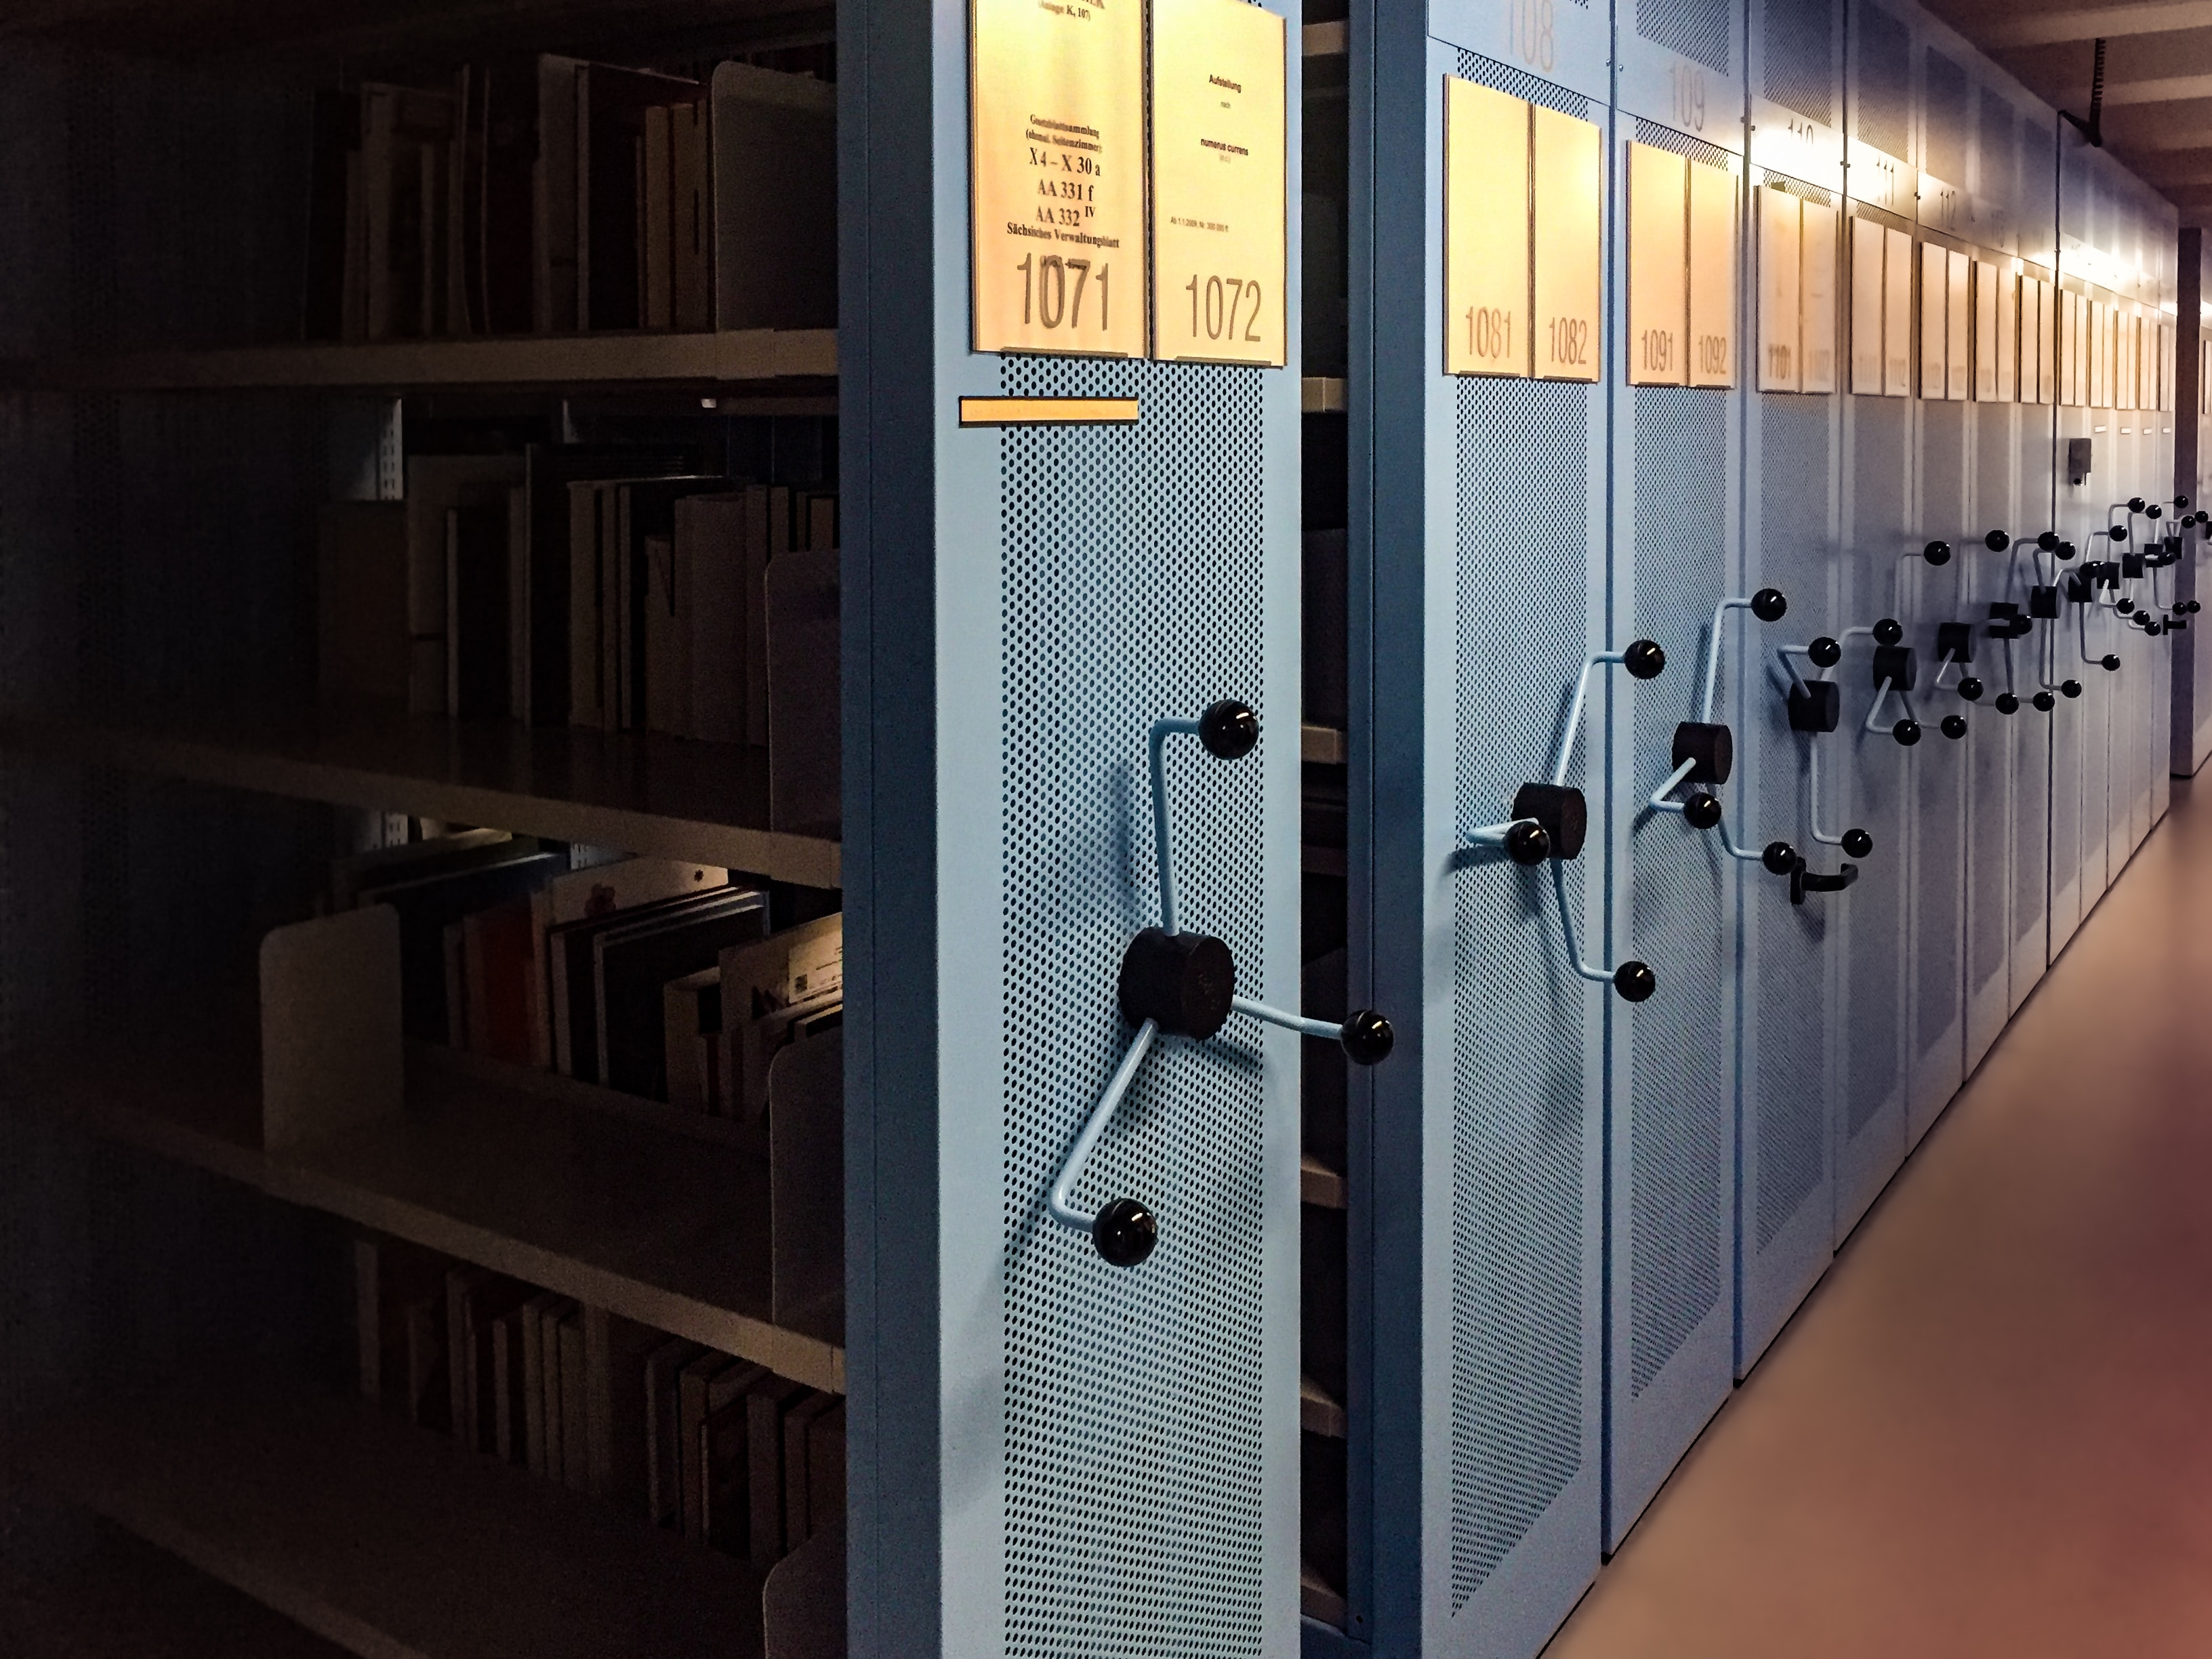
\includegraphics{pictures/archive-title-image}}%is only used with BFH-graphic and BFH-fullgraphic

%Activate the output of a frame number:
\setbeamertemplate{page number in head/foot}[framenumber]

\begin{document}

%    Was ist die Problemstellung Ihres Projektes
%   (Zielsetzungen, Anforderungen, Rahmenbedingungen)
%    Kilian
%    Wie wollen Sie die Problemstellung lösen?
%    (Architektur, Datenmodell, Prozessmodell, Technologien, usw.)
%    Nicolin
%    Wie setzen Sie das Projekt mit Scrum um?
%    Abidin Vejseli

    \setbeamertemplate{title page}[BFH-fullgraphic]
    \maketitle



    \begin{frame}{Table of Content}
        \framesubtitle{We will speak about:}
        \tableofcontents
    \end{frame}

    % Chapter one "Problem Statement"
    \section{Problem Statement}
    \setbeamertemplate{section page}[BFH-ruled]
    \frame{\sectionpage}

    \begin{frame}{Objectives}
        \framesubtitle{}
    \end{frame}

    \begin{frame}{Requirements}
        \framesubtitle{}

    \end{frame}

    \begin{frame}{General conditions}
        \framesubtitle{}
    \end{frame}
    %-------------------------------%

    % Chapter two "Solving the Problem"
    \section{Solving The Problem}
    \setbeamertemplate{section page}[BFH-ruled]
    \frame{\sectionpage}

    \begin{frame}{Architecture}
        \framesubtitle{Employing the MVC Pattern}

        \begin{columns} % Start the columns environment
            \begin{column}{0.5\textwidth} % Define the width of the left column
                \begin{itemize}
                    \item Modular design for easy extension.
                    \item Separate data, interface, and control flow.
                    \item Facilitates the potential addition of a GUI.
                \end{itemize}
            \end{column}

            \begin{column}{0.5\textwidth} % Define the width of the right column
                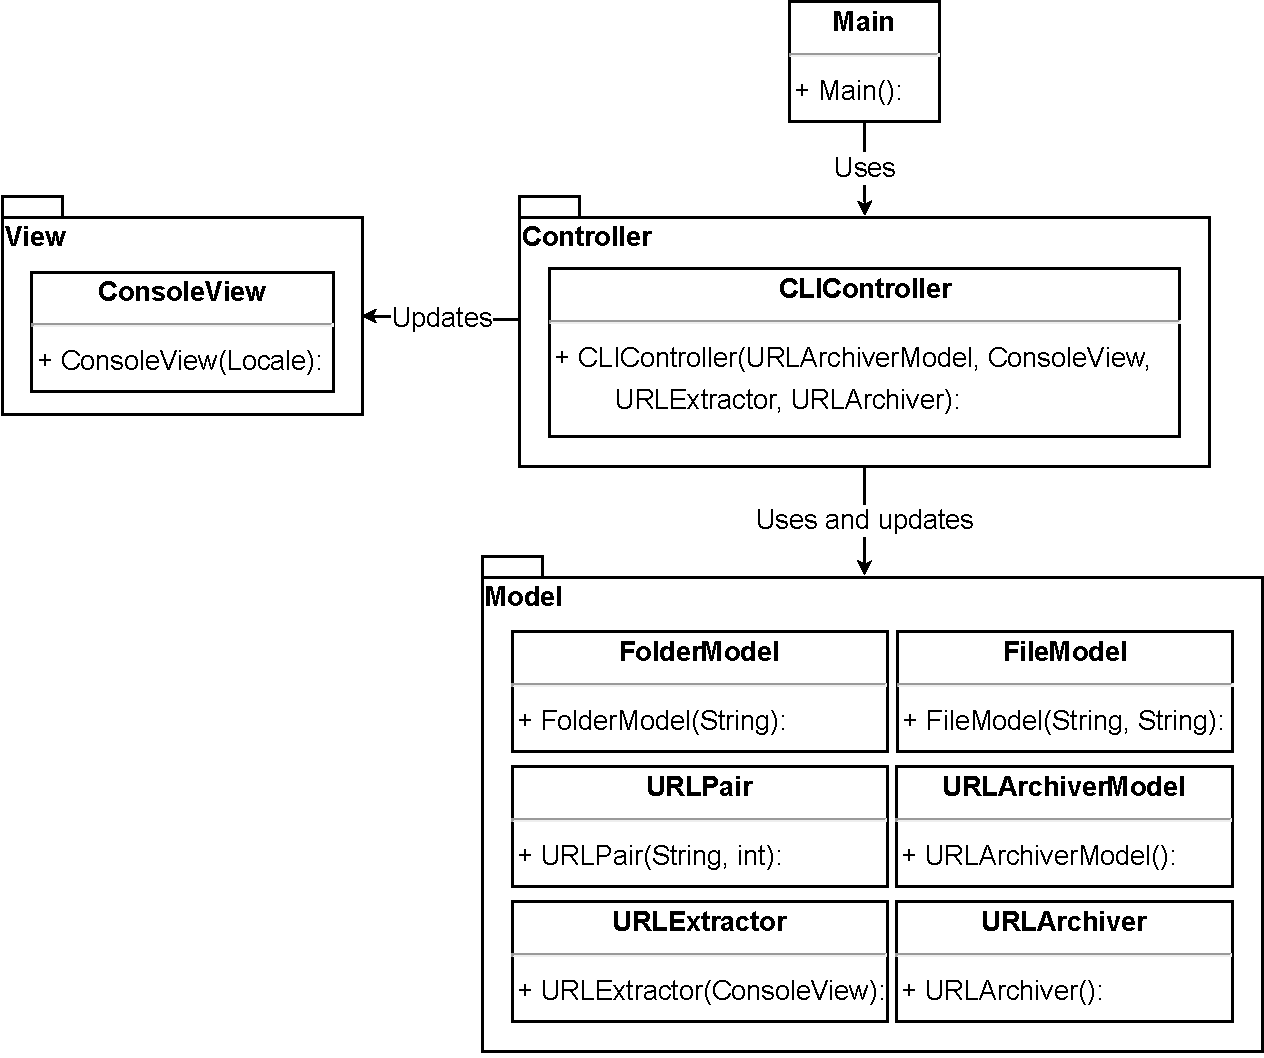
\includegraphics[width=1\textwidth]{pictures/mvc_diagram}
            \end{column}
        \end{columns} % End the columns environment
    \end{frame}

    \begin{frame}{Architecture}
        \framesubtitle{SOLID Principles}
        \begin{itemize}
            \item Scalable and robust design.
            \item Ensures maintainability and clear code structure.
            \item Commitment to best programming practices.
        \end{itemize}
    \end{frame}

    \begin{frame}{Architecture}
        \framesubtitle{Object-Oriented Approach}
        \begin{itemize}
            \item Promotes code reusability.
            \item Logical class hierarchies.
            \item Clear relationships between modules.
        \end{itemize}
    \end{frame}

    \begin{frame}{Architecture}
        \framesubtitle{Multilanguage Support with ResourceBundle}
        \begin{itemize}
            \item Ready for global adaptability.
            \item Future-proofing architectural choice.
            \item Potential to accommodate multiple languages.
        \end{itemize}
    \end{frame}

    \begin{frame}{Data model}
        \framesubtitle{Structured Data Logic}
        \begin{itemize}
            \item \textbf{FolderModel:}
            \begin{itemize}
                \item Represents a structured collection of files.
                \item Can throw a `FolderModelException` during invalid operations.
            \end{itemize}

            \item \textbf{FileModel:}
            \begin{itemize}
                \item Represents individual file data.
                \item Associated with `URLPair` objects.
                \item Can throw a `FileModelException` during invalid operations.
            \end{itemize}

            \item \textbf{URLPair:} Represents a pair of a URL and its related data.

            \item \textbf{URLArchiverModel:}
            \begin{itemize}
                \item Core model handling the archiving of URLs.
                \item Interacts with `URLExtractor` and `URLArchiver` utilities.
            \end{itemize}

            \item \textbf{UserChoice:} Captures user's decisions, possibly related to file operations or URL choices.

        \end{itemize}

        \textbf{Note:} These models ensure data integrity and consistency within our application, separating data handling from other concerns.

    \end{frame}

    \begin{frame}{Process model}
        \framesubtitle{Workflow for URL Extraction and Archiving}
        \begin{itemize}
            \item User can skip URLs, launch them, access help or quit the program at any time.
        \end{itemize}
        \vspace{0.8cm}
        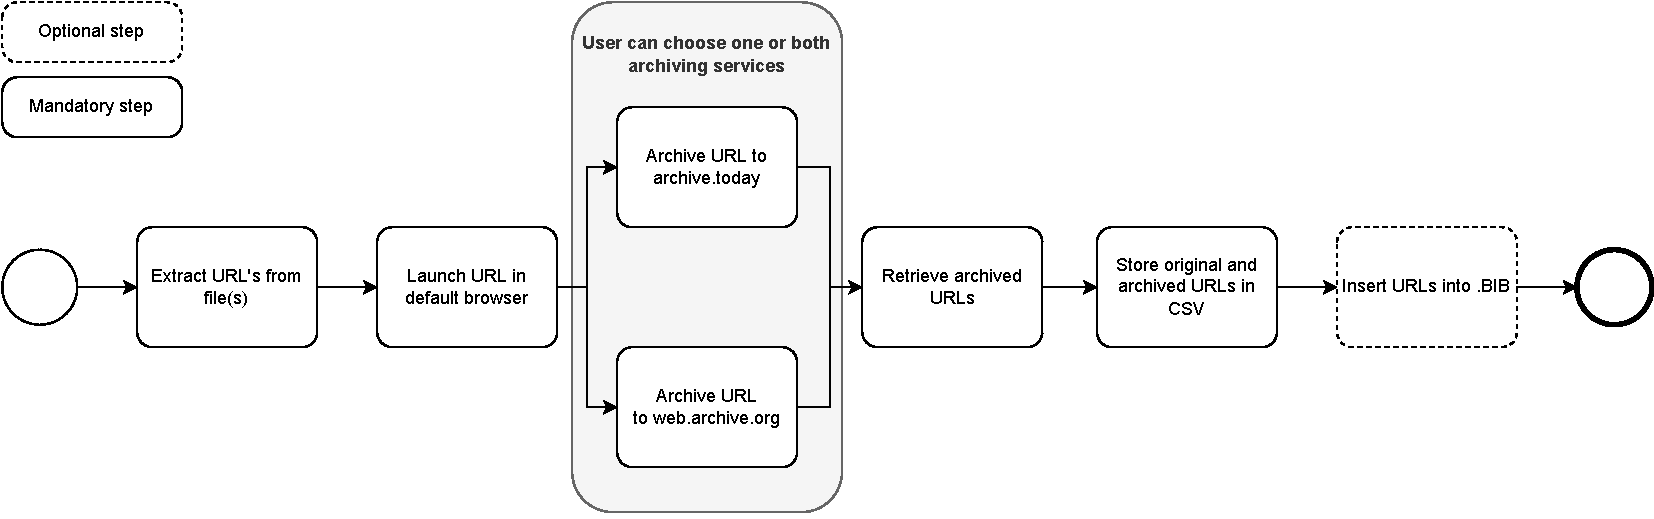
\includegraphics[width=1\textwidth]{pictures/process_model-simple}
    \end{frame}

    \begin{frame}{Technologies}
        \framesubtitle{}
    \end{frame}

    \begin{frame}{etc.}
        \framesubtitle{}
    \end{frame}
    %-------------------------------%

    % Chapter two "Project Management with SCRUM"
    \section{Project Management with SCRUM}
    \setbeamertemplate{section page}[BFH-ruled]
    \frame{\sectionpage}

    \begin{frame}{Scrum-Rollen}
        \framesubtitle{}
    \end{frame}

    \begin{frame}{Sprintziele}
        \framesubtitle{}
    \end{frame}

    \begin{frame}{Anforderungen}<
        \framesubtitle{}
    \end{frame}

    \begin{frame}{Scrum Adaptionen}
        \framesubtitle{}
    \end{frame}

    \begin{frame}{etc.}
        \framesubtitle{}
    \end{frame}
    %-------------------------------%

    \begin{frame}{Blocks}
        \begin{block}{Block with a title}
            Content.
        \end{block}
        \begin{block}{}
            Without title
        \end{block}
    \end{frame}

    \begin{frame}{Block types}
        \begin{exampleblock}{Exampleblock}
            Content.
        \end{exampleblock}
        \begin{alertblock}{Alertblock}
            Content.
        \end{alertblock}
        \begin{example}[Example environment]
            Content.
        \end{example}
    \end{frame}

    \section{section pages}
%These can be automaticlly called by using \AtBeginSection{\sectionpage}

    \setbeamertemplate{section page}[BFH-ruled]
    \frame{\sectionpage}

%Change base color scheme (option can be added)

    %\setbeamercolor{BFH}{parent=BFH-Orange}

    %\frame{\sectionpage}

    %\setbeamertemplate{section page}[BFH]

    %\frame{\sectionpage}

\end{document}

